% Use only LaTeX2e, calling the article.cls class and 12-point type.

\documentclass[12pt]{article}

% My packages

\usepackage{graphicx}
\usepackage{amsthm}
\newtheorem{mydef}{Definition}
\usepackage{dcolumn}
\usepackage{multirow}
\usepackage{booktabs}
\newcolumntype{d}{D{.}{.}{4.0}}
\newcolumntype{s}{D{.}{.}{1.4}}

% Users of the {thebibliography} environment or BibTeX should use the
% scicite.sty package, downloadable from *Science* at
% www.sciencemag.org/about/authors/prep/TeX_help/ .
% This package should properly format in-text
% reference calls and reference-list numbers.

\usepackage{scicite}

% Use times if you have the font installed; otherwise, comment out the
% following line.

\usepackage{times}

% The preamble here sets up a lot of new/revised commands and
% environments.  It's annoying, but please do *not* try to strip these
% out into a separate .sty file (which could lead to the loss of some
% information when we convert the file to other formats).  Instead, keep
% them in the preamble of your main LaTeX source file.


% The following parameters seem to provide a reasonable page setup.

\topmargin 0.0cm
\oddsidemargin 0.2cm
\textwidth 16cm 
\textheight 21cm
\footskip 1.0cm


%The next command sets up an environment for the abstract to your paper.

\newenvironment{sciabstract}{%
\begin{quote} \bf}
{\end{quote}}


% If your reference list includes text notes as well as references,
% include the following line; otherwise, comment it out.

\renewcommand\refname{References and Notes}

% The following lines set up an environment for the last note in the
% reference list, which commonly includes acknowledgments of funding,
% help, etc.  It's intended for users of BibTeX or the {thebibliography}
% environment.  Users who are hand-coding their references at the end
% using a list environment such as {enumerate} can simply add another
% item at the end, and it will be numbered automatically.

\newcounter{lastnote}
\newenvironment{scilastnote}{%
\setcounter{lastnote}{\value{enumiv}}%
\addtocounter{lastnote}{+1}%
\begin{list}%
{\arabic{lastnote}.}
{\setlength{\leftmargin}{.22in}}
{\setlength{\labelsep}{.5em}}}
{\end{list}}


% Include your paper's title here

\title{Computational hysteresis:\\ inter-task effects in human computation} 


% Place the author information here.  Please hand-code the contact
% information and notecalls; do *not* use \footnote commands.  Let the
% author contact information appear immediately below the author names
% as shown.  We would also prefer that you don't change the type-size
% settings shown here.

\author
{Edward Newell, Derek Ruths,\\
\\
\normalsize{\texttt{edward.newell@mail.mcgill.ca}}\\
\normalsize{\texttt{druths@networkdynamics.org}}\\
\normalsize{School of computer science, McGill University,}\\
\normalsize{3630 rue University, Montreal, Quebec, H3A 0C6, Canada}\\
\\
}

% Include the date command, but leave its argument blank.

\date{}



%%%%%%%%%%%%%%%%% END OF PREAMBLE %%%%%%%%%%%%%%%%



\begin{document} 

% Double-space the manuscript.

\baselineskip24pt

% Make the title.

\maketitle 



% Place your abstract within the special {sciabstract} environment.

\begin{sciabstract}

People still outperform sophisticated artificial 
intelligince systems in many tasks requiring general knowledge, 
qualitative judgment, and visuo-spatial reasoning. Recently, microtask 
platforms enable the programmer to import human judgment directly into 
algorithms: programs can post tasks, to be completed by users of such 
platforms in near real-time.
Some computer scientists consider microtask platforms to be a fundamentally
new computing architecture, but psychological effects can introduce systematic
bias. 
Here we investigate the effects that earlier tasks have on the results of 
subsequent ones, which we call \textit{inter-task effects}.
In a canonical image labeling task, we found that inter-task effects are
very strong---stronger than overtly framing tasks in terms of 
particular research goals.  However, in some cases, inter-task effects can
be leveraged to elicit more nuanced responses.
To study inter-task effects we introduce a framework that characterizes HPU 
bias in an application-independant way, based on its potential to alter an 
algorithm's path of execution.  Our findings suggest that careful consideration
should be given to inter-task effects when designing crowdsourcing studies. 

%microtask worker performs a series of tasks.  We find that early tasks can
%have a strong effect on later tasks, and that these effects can be stronger
%than those brought about by framing.
%
%course of human computation algorithms.
%application-independant quantity that measures the
%severity of priming.  We apply this framework to measure 
%
%in many
%tasks, especially ones requiring general knowledge about the world, qualitative
%judgment, and visuo-spatial reasoning.  Recently, microtask web platforms have 
%emerged. One can upload a batch of tasks to be completed by users who are paid 
%for their efforts.
%Though simple on the surface, these platforms dramatically enlarge the
%programmers toolkit: in effect they allow the programmer to import human 
%judgment into algorithms.  Some computer scientists consider
%such platforms to be a new computing architecture.  But people are very 
%different from electronic processors.  For example, context affects how a 
%person will respond to a prompt, and this complicates the formal treatment of 
%human computation.  To approach this issue, we introduce a framework 
%that quantifies the severity of priming in an application-independant way.
%We apply this technique to reveal an unforseen source of bias: the bias 
%induced by one task on another.  Surprisingly we find that 
%\textit{inter-task effects} introduce more bias than \textit{framing}, which
%has received more attention.
%
%more well-known 
%\textit{framing}, a more well-studied form of priming.
%
%Microtask platforms offer a fast, flexble, and inexpensive source of labour for
%clerical tasks \cite{Finnerty2013, chandler2013breaking, Berinsky2012351} and 
%recently have been adopted by researchers to augment datasets and solicit 
%participants \cite{paolacci2010running, Berinsky2012351, chandler2013breaking}.
%Computer scientists have described such platforms as a new computing 
%architecture, and seek to characterize “human co-processing units” (HPUs) in 
%analogy to CPUs and GPUs \cite{5543192}. However, it is known that people are 
%susceptible to 
%priming effects\cite{No2007,Swaab200299,Gopher2000308,sohn2001task,Ghuman17062008,BJOP1796,BJOP1826,Gass1999549}, which stands to complicate the HPU 
%perspective.  Here, we introduce a framework to recast this psychological 
%phenomenon as a kind of computational hysteresis. 
%We apply this framework to study \textit{inter-task effects} that arise when 
%microtask 
%workers perform a sequence of tasks. Surprisingly, earlier tasks can have a 
%very strong influence on workers during later tasks---stronger than overtly
%framing the tasks as serving different research goals.   
%This result has major implications for the design of crowdsourcing initiatives.
%The framework we introduce provides a general measure of priming severity, 
%and, in combination with machine learning tools, enables measurement without
%knowing ahead of time how priming will affect output.
\end{sciabstract}

\section*{Introduction}
Microtask crowdsourcing platforms like Amazon Mechanical Turk (MTurk) make it 
possible for requesters to submit batches of small tasks to a large pool of 
workers, who do the tasks for fun, a sense of purpose, and remuneration 
\cite{kazai2013analysis,Antin20122925}.  
Originally used to distribute clerical work, these platforms 
increasingly serve as a means to engage experimental 
participants in a research 
setting \cite{paolacci2010running,Berinsky2012351,snow2008cheap,alonso2009can}.
Typical tasks include tagging and categorizing images 
\cite{6116320,Zhai2012357}, transcribing voice recordings 
\cite{chandler2013breaking,paolacci2010running}
or handwritten notes \cite{Berinsky2012351,Finnerty2013}, and judging the 
relevancy of search results \cite{le2010ensuring,grady2010crowdsourcing,alonso2009can,kazai2013analysis}

These platforms make it possible to seemlessly integrate human and 
machine computation.  Researchers coined the term HPU 
(Human co-Processing Unit) in analogy to CPUs and GPUs \cite{5543192}.  
Attempts have been made to establish an HPU instruction set.  For example,
the X library provides function calls such as 
\texttt{X.vote()}, and \texttt{X.map()}
 \cite{little2010turkit,minder2011crowdlang,minder2012crowdlang,kittur2011crowdforge}.

Of course, there are obvious differences between HPUs and their silicone
counterparts.  When facing the same task, people do not generally
respond in the same way.  Common sense would dictate that a certain amount
of variability in responses made by people is inescapable.  But an important 
part of the variation is bound to be systematic, due to psychological or 
demographic factors.

Here, we highlight an important source of bias with
serious implications for any crowdsourcing initiative. 
It is known that people are susceptible to priming effects 
\cite{BJOP1796,No2007,beller1971priming}, and, in particular, task-repetition 
effects \cite{Gass1999549,sohn2001task}.  Thus, a worker's response during
one task may depend in part on previous ones.  Such \textit{inter-task} effects
would amount to a kind of \textit{hysteresis}, meaning that HPU outputs are not
only a function of the current input, but also of the history of inputs.  

There has been considerable investigation into the factors that affect the 
output from microtask work.  These include such factors as the 
level of 
pay \cite{kazai2013analysis}, training \cite{le2010ensuring}, pre-screening of 
workers \cite{paolacci2010running}, and user-interface design 
\cite{Finnerty2013}.  Researchers have also investigated \textit{framing}, 
by testing the effects of describing the workflow context 
\cite{Kinnaird2012281}, the purpose of tasks 
\cite{chandler2013breaking}, or using an alternative problem discription
\cite{thibodeau2013natural}.  To our knowledge, no study has investigated 
inter-task effects on microtask platforms.

We make two contributions towards understanding inter-task effects,
and systematic bias in HPUs in general.  First, we present a framework for 
quantifying bias in HPU outputs in terms of their potential impact 
algorithms.  This yields an approach for measuring the severity of bias 
that removes the need to understand the underlying psychological or 
demographic factors at play.  Second, we apply our framework to measure the
severity of inter-task effects on a canonical microtask: image labeling.

Using the  Amazon Mechanical Turk (Mturk) platform, we solicited workers to 
perform a series of image-labeling tasks.  We chose image labeling because it 
is one of the most common kinds of microtasks
\cite{chandler2013breaking,Berinsky2012351,Finnerty2013,paolacci2010running}, 
and it seems likely that this will remain the case in the long term because
of applications in computer vision research \cite{5543192}.
%In these tasks, workers labeled images featuring iconic cultural scenes,
%food, table-settings, and various utensils and cookware. 
We divided the tasks into an \textit{initial} and \textit{test} set, 
but, crucially, there was no distinction between these sets from the
perspective of the worker.  We varied the initial tasks, while 
keeping the test set the same, to analyze the effect of initial tasks on 
the labels provided during the test tasks.

As a point of comparison, we included treatments in which we induce 
\textit{framing}.
Before the workers labeled images, we indicated that the work 
was funded by a research lab with a particular area of interest, to see the 
influence this has on the workers’ subsequent labels. 
Surprisingly, inter-task effects were stronger than framing, in some cases 
about twice as strong. 
Our results demonstrate that initial tasks can change workers' focus in later 
tasks.  We also found that inter-task effects altered the level of specificity 
of worker's labels.  Our findings suggest that careful consideration should be 
given to the bundling of tasks when designing a study using a microtask 
platform.

\paragraph*{Computational hysteresis.}
Before describing our experiments, we dedicate some space to discussing
how we characterize and measure priming in HPU outputs.  Since HPU outputs are
stochastic, determining the effect of priming on an HPU population
amounts to determining the resulting change to the HPU population's 
distribution of outputs. 

To refine this, we distinguish between methods that determine \textit{whether}
two random sources have the same distribution 
(e.g. Pearson's chi squared test), from those that determine
\textit{the extent} of that difference (e.g. one of the many measures of 
statistical divergence).  We are interested in measuring the extent of
difference because our practical concern is the potential for such
differences to alter the course of an algorithm.

To measure the effect of some priming treatment, we must of course draw a 
comparison to some standard population.  In many cases, there may be an 
obvious comparison between a primed and unprimed population.  However, we 
refrain from proposing a canonical neutrally-primed HPU population; what is 
considered ``unprimed'' in one scenario may be ``primed'' in another. 
Instead, we speak of two HPU populations being \textit{differently primed}.

We present three alternative, equivalent definitions for the 
\textit{difference in priming} of two HPU populations, $\mathcal{P}$, and 
$\mathcal{Q}$, which we denote $\theta(P,Q)$.  To set up the definitions,
we will assume that $\mathcal{P}$ and $\mathcal{Q}$ 
were sampled randomly from the same initial population $\mathcal{R}$, and 
then were exposed to (possibly) different priming treatments. Then, the HPUs 
in $\mathcal{P}$ and $\mathcal{Q}$ perform some task, leading to popualtions 
of work-products, $P$ and $Q$.

The first definition provides the motivation for our choice of divergence
measure, because it directly measures the proportion of the time that a
binary decision will be changed due to priming effects:

\begin{mydef}
	\label{def:bias}
	{\upshape Maximum Bias:}
	Let $\mathcal{D}$ be a binary decision function, which takes a 
	work-product
	$r \in P \cup Q$ as input, and outputs a bit $\mathcal{D}(r)=b$, where 
	$b \in \{0,1\}$. Denote the \emph{bias} of $\mathcal{D}$, due to the
	different priming of $\mathcal{P}$ and $\mathcal{Q}$ by
	$\theta_\mathcal{D}(P,Q)$ and define it to be the difference 
	in the expected output of $\mathcal{D}$ when acting on work-products from 
	$P$ and $Q$:
	$$
	\theta_\mathcal{D}(P,Q) = 
		\left| 
			\mathrm{E}\left\{ \mathcal{D}(p) \right\} 
			- \mathrm{E}\left\{ \mathcal{D}(q) \right\} 
		\right|,
	$$
	where $p \in P$, $q \in Q$.  Then, define the difference in priming 
	between $\mathcal{P}$ and $\mathcal{Q}$ to be the worst-case bias, i.e. 
	the bias of the most susceptible decision:
	$$
	\theta(P,Q) = 
		\sup_\mathcal{D} \theta_\mathcal{D}(P,Q)
	$$
\end{mydef}
If $\mathcal{D}$ is the condition of an \texttt{if}-statement, then the 
definition above is the change in the fraction of the time that a given 
path of execution is followed due to HPU priming.

While this is precisely what we want to measure, it is not at all clear how
to go about doing it.  The second formulation provides a practical connection
by rephrasing priming in terms of its distinguishability:

\begin{mydef}
	{\upshape Distinguishability:}
	Let $\mathcal{D}$ be a distinguisher algorithm, which takes work-product 
	$r \in P \cup Q$ as input, and outputs a \emph{guess} 
	$\mathcal{D}(r) \in \{0, 1\}$. Now define a validation test 
	$V(\mathcal{D}, R_0, R_1)$ as follows. A bit is drawn uniformly at random, 
	$b \in_R \{0, 1\}$, and then a work-product $r$ is chosen uniformly at 
	random from one of the populations, decided by the bit: $r \in_R R_b$. 
	Input $r$ into $\mathcal{D}$, and if $\mathcal{D}(r) = b$, we say 
	$\mathcal{D}$ \emph{guessed correctly}, and the value of $V$ is 1, 
	otherwise $V = 0$.

	A distinguisher that guesses randomly will still be correct half of the 
	time. Therefore, denote the performance of $\mathcal{D}$ by 
	$\eta_\mathcal{D}(P, Q)$, and let
	$$
		\eta_\mathcal{D}(P,Q) = 2\cdot \mathrm{E}\{V(\mathcal{D},P,Q)\} - 1.
	$$
	Then define the difference in priming between $\mathcal{P}$ and 
	$\mathcal{Q}$ to be the performance of the best possible distinguisher:
	$$ 
		\theta(P,Q) = \sup_\mathcal{D} \eta_\mathcal{D}(P,Q)
	$$
	\label{def:dist}
\end{mydef}

\textbf{Definition 2} relates the difference in priming to the 
\textit{optimal Bayes classifier} for determining whether a given HPU output
came from $P$ or $Q$.  This means that we can obtain a lower bound on
$\theta(P,Q)$ based on the performance of an actual classifier, which provides
recourse when purely statistical methods fail.

The statistical divergence measure underlying the previous definitions is the
divergence measure known as the ``total variational distance'' or 
$l_1$-distance:
\begin{mydef}
	\label{def:l1}
	{\upshape Total variational distance $\theta_{l_1}$:}
	Define the difference in priming between $\mathcal{P}$ and $\mathcal{Q}$ 
	to be equal to the total variational distance between the work-products 
	$P$ and $Q$:
	$$
	\theta_{l_1}
	= \sup_{A \subset \mathcal{X}} \left| \sum_{x \in A} f_P(x) - f_Q(x)\right|
	= \frac{1}{2} \sum_{x \in \mathcal{X}} \left| f_P(x) - f_Q(x) \right|,
	$$
	where $f_P(x)$ denotes the probability of observing x when sampling from P.
\end{mydef}
The equivalent formulation for $\theta(P,Q)$ in 
\textbf{definition \ref{def:l1}} provides a grounding in a fundamental
measure of statistical divergence, and a connection to information theory.  
The equivalence of the three definitions
follows from the known fact that no algorithm can have output that differs
on inputs $P$ and $Q$ more than $l_1 \times 100\%$ of the time.  We provide
proofs in the supplementary material.

The difficulty of measuring $\theta(P,Q)$ depends on what the universe of
possible outputs are, as well as how $P$ and $Q$ are actually distributed,
both of which are mainly determined by the task that the HPUs are asked to 
perform.  In the case where workers label an image with a free-text input, 
the number of different possible labels can be in the thousands or more.  If
the support, $\mathcal{X} = P \cup Q$, is large compared to the number of 
HPU outputs sampled, so that many labels appear only once (which in any case
is expected from Zipv's law), then estimating $\theta$ directly from the
observed frequencies of labels is difficult.  

One approach to estimating the $l_1$-distance from samples, which appears
reasonable on the surface, is to use the observed frequencies of each output
$x$ from $P$ and $Q$ to estimate $f_P(x)$ and $f_Q(x)$, and calculate 
$\theta(P,Q)$ directly from \textbf{definition 3}.  This is the so-called naive
approach to estimating $l_1$-distances, and is aptly named because it tends
to produce very inflated values.  More recent techniques have for estimating
$l_1$ have been suggested by Valiant \cite{val-thesis}, and Batu 
\cite{batu2000testing,batu2013testing}.  We reserve the discission of these
techniques to the supplementary material; they do not turn out to be useful
because they do not provide confidence intervals.  Thus our only recourse is
to test the performance of classifiers at distinquishing $p \in P$ from 
$q \in Q$, which allows us to estimate a lower bound on $\theta(P,Q)$.  This 
turns out to be sufficient, and has the advantage that, so long as they are
learnable, it is not necessary to understand exactly how $P$ and $Q$ differ.


\paragraph{Experimental setup.}
We performed two experiments, soliciting respectively 900 and 2300 MTurk 
workers to label images depicting iconic cultural scenes, meals, ingredients, 
table-settings, and various utensils and cookware. In these experiments,
workers were randomly assigned to treatments, and depending on this 
assignment, were exposed to different framing primes, given a different 
set of initial images, and shown a different permutation of the test images. 
For both experiments, workers were first shown brief instructions.  
The framing prime was then shown, unless the given 
treatment involved no framing.  Workers then performed a series of 
image-labeling tasks and had to provide five labels per image. 
For the purpose of analysis, we denote the first five images as the 
\textit{initial set}, and the last five as the \textit{test set}, but no
distingction was made from
the perspective of the worker.
Table 1 sumarizes the various experimental treatments for both 
experiments.

\begin{table}[t]
\centering
	\begin{tabular}{ l  l  l }
		\hline                       
		Treatment & Framing prime & Initial image set	\\ 
		\hline                       
		\textit{Experiment 1}\\
		$\textsc{ambg}$ & None & Ambiguous\\
		$\textsc{img:cult}$ & None & Cultural\\
		$\textsc{img:ingr}$ & None & Ingredients\\
		$\textsc{frm:cult}$ & Cultural & Ambiguous\\
		$\textsc{frm:ingr}$ & Ingredients & Ambiguous\\
		\hline  
		\textit{Experiment 2}\\
		$\textsc{img:food}$ & None & Food\\
		$\textsc{img:obj}$ & None & Objects\\
		$\textsc{frm:food}$ & Food & None\\
		$\textsc{frm:obj}$ & Objects & None\\
		\hline  
	\end{tabular}

	\caption{ \footnotesize{ 
		Workers were uniformly randomly assigned to one of the 
		treatments listed above. 
		The full funder names used were 
		Cultural: ``The Global Foundation for Cultural Recognition'' and 
		Ingredients: ``The National Foundation for Nutritional Awareness''.  
		The ambiguous, cultural, and ingredients initial image sets are shown 
		in \textbf{Figs. 2}, \textbf{3}, and \textbf{4}.
	}}
	\label{table:1}
\end{table}

\begin{figure}
	\centering
	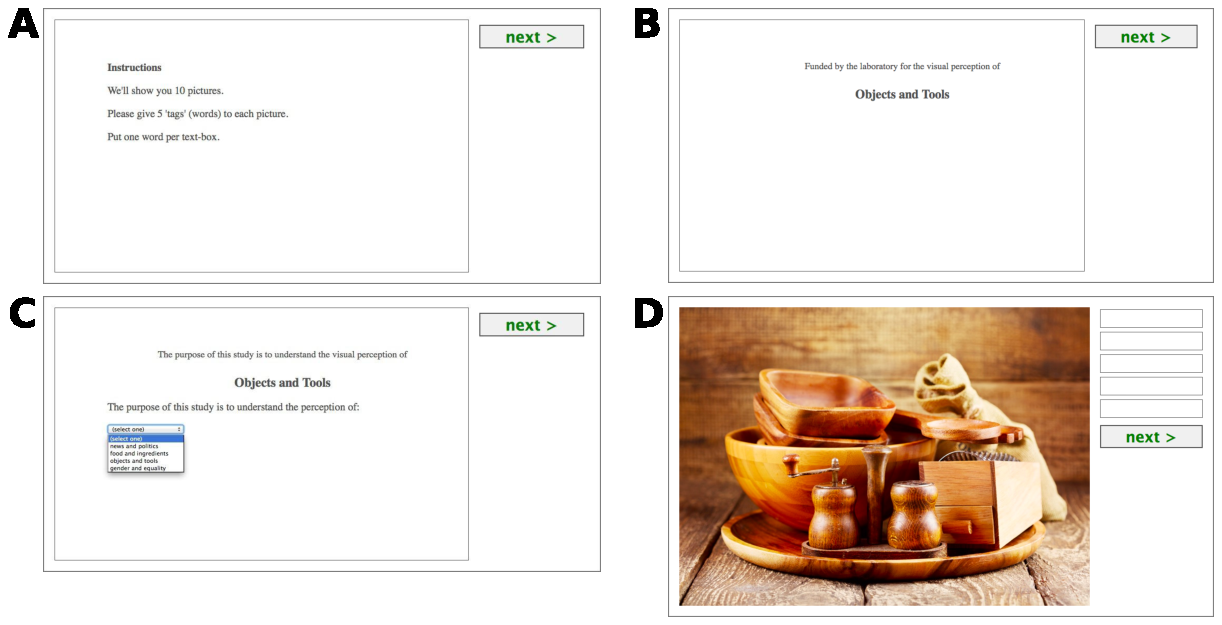
\includegraphics[scale=0.7]{figs/tasks.pdf}
	\caption{Examples of slides used for the image labeling tasks. A) instructions shown to all workers; B) a framing slide; C) a slide from the initial set for treatment IMG:FOOD; D) a slide from the initial set for treatment IMG:OBJ; E) a slide from the test set shown in all treatments. The full set of slides used for all treatments is presented in the supplementary material.}
	\label{fig:task}
\end{figure}


\paragraph{The strength of inter-task effects.}
\begin{figure}
	\centering
	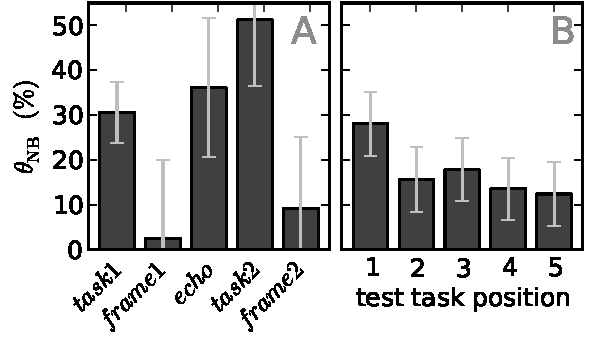
\includegraphics[scale=1]{figs/theta.pdf}
	\caption{
		Difference in priming observed for various pairs of worker populations.
		The pairs of populations differed in terms of the initial tasks they
		performed (bars labeled by \textit{inter-t.}) or in terms of the framing
		to which they were exposed (bars labeled by \textit{frame}; see table 1 for
		details about the treatments).  The difference in priming was 
		measured based on the accuracy of a naive Bayes classifier in 
		resolving which treatment workers belonged to, as described in the 
		text.  
	}
	\label{fig:theta}
\end{figure}


%\paragraph{Dynamics of inter-task effects}
%\begin{figure}
%	\centering
%	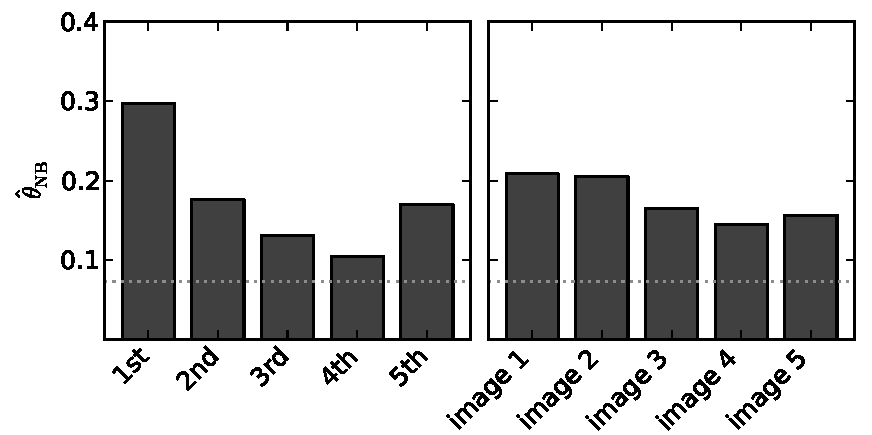
\includegraphics[scale=0.7]{figs/theta_by_pos_img.pdf}
%	\caption{
%		Difference in priming observed for various pairs of worker populations.
%		The pairs of populations differed in terms of the initial tasks they
%		performed (bars labeled by ``inter-t.'') or in terms of the framing
%		to which they were exposed (bars labeled by ``frame''; see table 1 for
%		details about the treatments).  The difference in priming was 
%		measured based on the accuracy of a naive Bayes classifier in 
%		resolving which treatment workers belonged to, as described in the 
%		text.  
%	}
%	\label{fig:theta_pos_img}
%\end{figure}

We analyzed the overall strength of inter-task effects and framing, by looking
at pairs of treatments that performed the same test tasks, but had done
different initial tasks or had been exposed to different framing.
For each such pair, we assessed the performance of classifier
in predicting which treatment workers belonged to, based on the labels they
provided during the test tasks (see fig 2).  
Based on \textbf{Definition 2}, this is a lower bound on the amount 
bias introduced by the initial tasks and framing.

In experiment \textit{inter-t.1}, the test tasks required workers to
label relatively cluttered images of table settings, which had various items
of food, utensils, dishware, and other objects natural to such settings.
For one treatment, the images in the initial tasks consisted exclusively of 
food, and for the other, they consisted exclusively of non-food objects, 
particularly cookware and utensils.  We saw a strong effect of priming, 
based on the classifier performance (see fig. 2). 

In a related experiment, \textit{frame1}, workers were given the same test tasks
as in \textit{inter-t.1}, but were either told 
that ``The purpose of this study is to understand the viusual perception of
Food and Ingredients'' or ``\ldots of Objects and Tools''.  This overt framing
of the task in terms of a specific research objective had remarkably milder
effects on workers than the initial tasks (see fig. 2).

We performed another set of experiments based on a different set of test 
tasks, and where the initial tasks and framing were directed along a different
conceptual axis.  In \textit{inter-t.2} and \textit{frame2}, the images in the test 
tasks displayed prepared meals from a variety of ethnic backgrounds.  We then
designed the framing and initial tasks to focus either on food or cultural 
elements.  In the previous experiments, the primes were always focused on 
concrete ``highly imageable'' concepts (food and objects), these experiments
mixed a concrete concept (food) with an abstract concept (culture).
The initial tasks in \textit{inter-t.2} either depicted prepared meals (but having
ambiguous cultural association), or iconic cultural scenes (including music, 
dance, and sport).  Workers in \textit{frame2} were told that the ``This study
was proudly funded by the National Foundation for Nutritional Awareness'' 
or the ``\ldots Global Foundation for Cultural Recognition''.

The results for \textit{inter-t.2} and \textit{frame2} confirmed that 
inter-task effects are much stronger than framing (see fig. 2).  In fact, 
intertask effects were even stronger in this experiment than the previous.

\paragraph{Sufficiency of framing.} Given just how much stronger
inter-task effects were, the reader may wonder whether the framing was 
in some sense ``sufficient''.  
We designed our framing tasks based on
work that had previously studied framing effects in micro-task settings.  
Prior studies have shown that framing the purpose of a task, or indeed, 
simply changing a single, seemingly non-critical word in a task description, 
has significant effects on worker's resonses.  Perhaps more importantly, the 
framing treatments were included to provide a reasonable basis for comparison,
and it is clear from our results that the prior tasks performed by a 
worker are much stranger than the effects induced by descriptions of a task's
purpose, or the requester's mandate.

Nevertheless, we included one more experiment, \textit{frame*3}, to test the 
effect of framing when the worker is required to \textit{echo} the framing 
statement.  \textit{frame*3} was based on \textit{frame2}, but the worker
had to indicate, using a menu option, what the purpose of the study was,
before they could proceed.  In one sense, this seems to go beyond what one
might mean by ``framing''.  By forcing the worker to echo the frame, we provide
a clear indication that the frame is a particularly important detail, 
elevating its importance above even the instructions that had been provided
beforehand.

The framing effect in \textit{frame*3} was quite strong, being on par with the
inter-task effects we had observed (see fig. 2).  We are not sure whether
the \textit{frame*3} should be considered framing,
or whether it should be considered as an instruction, or perhaps as a 
screening-task.  Regardless, our results show that worker's responses are 
profoundly affected by recently completed tasks. 


\paragraph{Dynamics of intertask effects.} 
In the results shown above, we considered the aggregate effect that the
first five initial tasks had on the last five test tasks.  But it would stand
to reason that the first test task might be
most strongly influenced, and that, as the worker proceeds, the intervening 
test tasks would tend to wash out the priming induced by the initial tasks.

One complication to this is the fact that the strength of intertask effects
should also depend on the task: that is, workers performing one task are not
necessarily as susceptible to inter-task effects as when performing another 
task.  To account for this, we performed five replicates of the 
\textit{inter-t.1} experiment, each using a different permutation of the 
test tasks.  We ensured that each test task appeared in each of the 
five possible relative positions.  This allowed us to measure the inter-task
effects as a function of task position, independant of the particular image
used in the task (see fig. 2B).  We found that, as one would expect,
the first test task tends to be the most strongly affected.  The effect drops
considerably for the second task, and continues to fall for the third and 
fourth.  Interestingly, the last test task consistently showed a small increase
in priming effect.  We also observed this in \textit{inter-t.1}. 
We do not know the psychological mechanism behind this phonomenon, but we 
speculate that, since the worker knows that there are ten tasks in total,
they might reflect on the task overall batch of tasks as they near the end,
and in so-doing might partially re-activate the influence of the initial tasks.

While the strength of inter-task effects appeared to depend strongly on
the position of the task, it was considerably less dependant on exactly what
was in the task (see fig. 2C).  To be sure, we intended for the tasks to be 
similar, and it does appear that the various test tasks had similar 
susceptibilities to inter-task effects.

\paragraph{Initial tasks' affect on the direction of focus} 
\begin{figure}
	\centering
	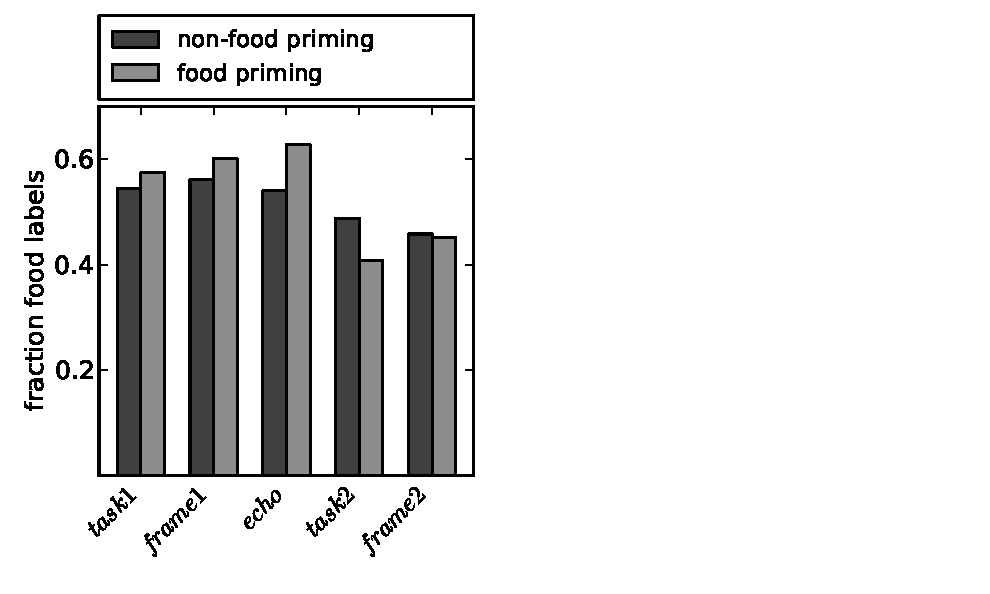
\includegraphics[scale=1]{figs/food_specificity.pdf}
	\caption{
		Difference in priming observed for various pairs of worker populations.
		The pairs of populations differed in terms of the initial tasks they
		performed (bars labeled by \textit{inter-t.}) or in terms of the framing
		to which they were exposed (bars labeled by \textit{frame}; see table 1 for
		details about the treatments).  The difference in priming was 
		measured based on the accuracy of a naive Bayes classifier in 
		resolving which treatment workers belonged to, as described in the 
		text.  
	}
	\label{fig:food_specificity}
\end{figure}

At this point we have only discussed priming effects in terms of a 
classifier's ability to detect them.
We have said nothing qualitative about the \textit{nature} of these effects.  
This demonstrates an advantage of using classifiers to measure priming.  
Machine learning algorithms are designed to find salient differences 
by generalizing, inductively, from examples, so one
need not know beforehand how workers were primed, nor the natuer of the  
priming effects.  Machine learning algorithms are specifically designed to 
generalize inductively from examples, which makes
it possible to estimate how different two populations with little prior 
knowledge.

But once having shown that workers are strongly primed by initial tasks, it is
natural ask whether workers were biased to provide labels that reflected, 
in some way, the \textit{content} of the initial tasks.  The conceptual basis
for the primes in experiment 2 were eithre \textit{food} or 
\textit{objects and tools}.  Thus, we can test whether workers exposed to food
primes produced more food-related.  

To identify food-related labels, we used the wordnet corpus.  Wordnet
is an extensive corpus for English, that includes hypernym-hyponym 
relationships between words.  The hypernym relation correpsonds to conceptual
abstraction.  For example \textit{bread} is a hypernym of 
\textit{pumpernickel} because pumpernickel is a \textit{type of} bread.
The hyponym relation is simply the converse: pumpernickel is a hyponym
of bread.  For the purpose of our analysis, when we refer to hypernyms,
we will mean both direct hypernyms, as well as the hypernyms of hypernims,
and so on, with an analogous interpretation for hyponyms.

We collectod a small set of top-level food-related nouns in wordnet,
together with all of their hyponyms, and took the resulting set of 
3589 lemmas as an operational definition for the set of English food-related 
words.  This set is quite extensive, containing somewhat obscure forms such as
``burgoo'' and ``barmbrack'', and consumables at the fringe of what might
be considered food such as ``vitamin B'' (or if you prefer, 
``B complex''), as well as more common lemmas like
``banana'',  ``bread'', and of course ``banana bread''.  We found that,
for the data in experiment 1, this method produced excellent aggreement with 
human annotation of food-related words (see supplementary material).  
For the analysis exp2, the variety of non-English names for ethnic dishes 
forced us to rely on a manual approach.  This corroborated our results
for exp1, and we encourage the interested reader to read our discussion of
the manual approach in the supplementary material.

Our findings matched the straightforward expectation that workers exposed to 
food related-primes were biased to provide more food-related labels during 
test tasks (see Fig. 3A).  Had we relied on the intuition that workers 
should be biased to label according to the underlying concept of their prime,
we would have underestimated the strength of priming effects.  This
again illustrates the advantage of using classifiers to detect priming as
opposed to testing for the effects that one might intuitively expect.  
Though present, the expected influence on the number of food-related words
cannot account for the bulk of inter-taks effects.

\paragraph{Effects on label vocabulary.}
Inspecting the labels manually, one striking observation was that in
\textit{test-t.2}, workers that initially images of cultural scenes seemed
more likely to give generic labels, compared to those that initially labeled 
images depicting prepared meals.  Recall that, for these treatments, the test 
tasks contained images depicting prepared meals, which are very similar in
content to the initial tasks for the latter set of workers.  Workers that
had already labeled 5 images depicting food were less likely to attribute
the generic label ``food'' during the first test task, doing so only 16 times,
compared to 76 times by workers that had labeled culture-related images 
containing no food.  This observation suggests that, when workers label a 
series of very similar images.

One straightforward way to test whether workers from exp2.task.food are 
being more specific than those from exp2.taks.cult is to look at the number 
of unique labels they provided for each image.  Workers attributing more
specific labels should produce a larger vocabulary of unique labels for a 
given, which is indeed what we found (see Fig. 3B).  Workers from 
exp2.task.food produced as much as 33\% more unique labels per image than 
workers from exp2.task.cult, and the relative excess of the vocabulary size
followed the general trend of inter-task effects that we observed in 
Fig. 2B.

To confirm our expectation that the larger vocabulary corresponds to a 
the use of \textit{more nuanced} words, we used the 
hypernym-hyponym of wordnet to operationalize a notion of relative 
specificity.  We define the relative specificity of two sets of labels $P$ 
and $Q$ as:
$$
	S(P,Q) = \frac{1}{|P \times Q|}\sum_{p \in P} \sum_{q \in Q} 
		\left(\mathbf{1}_{[p>q]} - \mathbf{1}_{[q>p]}\right),
$$
where $\mathbf{1}_{[p>q]}$ evaluates to 1 if $p$ is a hyponym of $q$.
Using the above equation, we found that, for every images in the 
test set, the labels attributed by workers in exp2.task.food were more 
specific than those by workers in exp2.task.cult.

Thus, when workers perform a series of similar image labeling tasks it would
appear that they tend to avoid generic words, opting instead for more specific
ones, and yielding a richer vocabulary of labels.  Qualitative 
characterisation and classification is one of the most comman applications of 
microtask platforms, and this finding suggests that bundling similar tasks 
together substantially increases the specificity of HPU output. 

Our observations of the effects on specificity would appear to be consistent
with the phenomenon of negative priming.
Negative priming occurs when a person becomes desensitized to non-salient 
stimuli to which she is repeatedly exposed. Consider that, workers that 
initially labeled images depicting prepared meals might no longer
regard the generic labels \texttt{food} or \texttt{meal} to be salient, and 
opt instead for \texttt{bread}, or \texttt{pasta}.  But for workers that
initially labeled cultural images, these rather generic labels might well seem
appropriate.
 
We are suggesting that, although workers are not instructed to compare images 
in any way, prior tasks nevertheless create a frame of reference relative to 
which later tasks are judged. This in turn influences the perception of 
salience. Thus, in a series of subjective characterization tasks that have 
very similar content, workers' focus will tend to be directed away from 
generic, shared attributes, towards those attributes that are specific and 
distinguishing.

To see how the initial tasks and the framing affected 
the focus of the workers' labels, we classified all the labels provided
on test tasks as either \texttt{culture}, \texttt{food}, \texttt{both}, or 
\texttt{neither} (we describe the label classification method in more detail
in the supplementary material).  Focusing on the labels provided to the first 
test task,
workers that had initially labeled cultural images provided far more cultural
labels during test tasks, and fewer food labels, than workers that initially
labeled images depicting ingredients (see \textbf{Fig. 2}).  On the other 
hand, the framing primes had no statistically significant effect.


\begin{table}
\centering
\begin{tabular}{ l  s s s s}

\toprule    
Image set   
& \multicolumn{1}{c}{Ambig.} 
& \multicolumn{1}{c}{Cultural} 
& \multicolumn{1}{c}{Ingr.}
& \multicolumn{1}{c}{Test} \\
  
\midrule

Ambiguous  & 1 & 0.0418 & 0.142 & 0.167 \\

Cultural  & 0.0418  & 1 & 0.0347 & 0.0561 \\

Ingredients  & 0.142  & 0.0347 & 1 & 0.110 \\

Test & 0.167  & 0.0561 & 0.110 & 1
\\
\bottomrule

\end{tabular}
\caption{\footnotesize{
Pairwise similarities of each image set based on the labels attributed to them (see \textbf{Eq. 4}).
}}
\label{table:2}
\end{table}

One weakness of the above analysis is the reliance on the informal notion
of the similarity of one set of images to another. The 
characterization of image content is a deeply complex issue that has been 
approached by many disciplines \cite{panofsky1939studies,shatford1986analyzing,Tversky1977327,Jaimes20002}. \textit{Perceptual similarity} is a 
particularly recalcitrant concept.   But to formalize our claim, we seek a 
measure of similarity between two sets of images, 
\textit{with respect to the labeling task}.  This can be operationalized
in a straightforward way, by using the similarity of the labels given to images
as a proxy for the similarity of the images.  Thus, to measure the 
similarity between two sets of images, X and Y , we computed the Jacquard 
index between the sets of labels attributed to them:
$$
	\mathrm{Sim}(X,Y) = \frac{L(X) \cap L(Y)}{L(X) \cup L(Y)}
$$
where $L(X)$ denotes the set of labels attributed to images in $X$.

The pairwise similarities of the image sets are presented in Table 2. This 
shows that the workers that yielded higher specificity labels were from 
treatments whose initial tasks were more similar to the test tasks (c.f.
\textbf{Fig 3}).

Such a phenomenon would be consistent with the psychological mechanism known as
\textit{negative priming}.
\paragraph{The role of task position in inter-task effects.}
Up to this point, we have focused on the inter-task effects induced on 
the first test task.  Not suprisingly, this task was, in general, more 
strongly affected than the others.  It would stand to reason that, as workers 
proceed through the test images, priming induced by the initial tasks would
be ``washed out'', and replaced by the effects of the test tasks themselves,
which do not differ between treatments.

To investigate this, we performed a second experiment, in which we permuted
the test tasks in such a way that every test task appears in each of the
5 locations equally often.  This allows us to track the intertask effects for
a given test task as it is rotated through the five positions.  Workers were
again given one of two initial sets of tasks, which either involved labeling
utensils, cookware, and table settings (but no food), or isolated close-up
images of prepared meals.  We measured the performance of a Naive Bayes 
classifier in distinguishing whether labels attributed to a given test 
image were provided by a worker that labeled objects or meals, as shown in 
\textbf{Fig. 4}.

The strength of inter-task effects show a clear trend based on the position of
the test task.  We see that, in general, the first test image is most severely
affected, and the severity of effect drops off.  Curiously, the severity then
rises again for the second last, and, especially, final test image.  We 
speculate that this is related to the workers being aware that they are 
reaching the end of the batch of labeling tasks.  To be transparent about the
rate of compensation, we informed workers that they would complete a total
of ten image-labeling tasks.  Perhaps as the worker nears the end of the batch
of tasks, she reflects on the overall experience, and in activating the
memory of the early tasks, is partially re-primed.


\paragraph{Conclusions.}
Our results show that inter-task effects can have a strong influence on how 
workers label images. In particular, we observed that prior tasks influence 
the specificity and content of labels. Surprisingly, framing a task by 
indicating a semantically-loaded funder had much milder effects on worker 
outputs, generally below the statistical power of our tests.

We therefore caution those designing studies using human computation: even if 
the requester has eliminated surrounding influences to every practical extent, 
\textit{the greatest source of bias might lurk in the tasks themselves}. Due 
consideration should be given to how tasks are bundled together. While our 
measurements of $\hat{\theta}_\mathrm{NB}$ indicated that inter-task effects 
persisted even to the fifth test image, the most severe effects arise between 
consecutive tasks.

Our proposed priming definition yields general purpose measure of priming 
effects. We used three approaches to detect priming effects: 1) using a Naive 
Bayes classifier to measure $\hat{\theta}_\mathrm{NB}$, 2) tallying the 
number of culture- and food-oriented labels, and 3) comparing the relative
specificity of labels based on an ontology. Of the three, $\theta_\mathrm{NB}$ 
was the most sensitive.

In one sense, this is not surprising because the Naive Bayes classifier takes 
into account the frequency of occurrence of all labels encountered during 
training. But it is remarkable that the method which incorporates neither 
prior knowledge about the image contents nor label semantics, outperforms 
those that do. This is a powerful feature because, given the outputs from two 
sets of workers, one can test whether they have been differently primed 
without knowing how that priming might manifest.

Our algorithmic definition of priming is phrased in terms of worker outputs 
rather than psychological phenomena. This provides a connection between the 
priming effects and their potential to impact decisions made on the basis of 
worker outputs. In the case of a 1-bit binary decision, $\theta$ describes the 
worst-case bias introduced by failing to control for priming effects.

Batching similar tasks together appears to yield higher more specific HPU 
outputs. Our proposed connection between similarity and specificity during 
image-labeling might be used to tune the specificity of labels. For example, 
If one seeks very nuanced labeling, our results suggest that the images 
should first be sorted into batches based on their similarity. This could be 
accomplished by beginning with a first, coarse labeling of unsorted images, 
followed by bundling based on the similarity of coarse labels. Then, bundles 
of similar images could be served for a second round of finer labeling. The 
sorting and re-labeling could in principle be repeated.

Such a workflow involves serial processing, which points to an interesting 
possible differ- ence difference between HPUs and CPUs. In general, whenever 
an aspect of a problem can be parallelized when employing CPUs, one gains 
efficiency. But here, because of HPU hysteresis, one might gain precision by 
using HPUs with a more serialized algorithm. Further testing is needed to 
determine the gain in precision from this approach.


\bibliography{newbib}
\bibliographystyle{Science}



\end{document}




















%Next we observed how inter-task effects on label composition (i.e. food- vs 
%culture-oriented labels) evolve as workers proceed through test images. We 
%define the excess cultural orientation as the number of culture-oriented 
%labels minus the number of food oriented ones. To meaning- fully compare the 
%excess cultural orientation between test images, we must, however, account 
%for the fact that some images inherently carry more cultural content than 
%others. In keeping with our notion of priming difference, we calculate the 
%excess cultural content for both CULTimg and
%
%AMBG, and take their difference to be the relative excess cultural content, 
%$\Delta_{cult}$. Formally,
%
%		*** Formula for delta cult\ldots
%
%where $N^(i)_{w,cult}$ stands for the number of culture-oriented labels 
%attributed by worker w to image i, while $N^(i)_{w,food}$ similarly counts
%food-oriented labels, and $N$ is the total number of labels in a treatment.
%
%We found $\Delta_{cult}$ was largest for the first test image, but dropped off 
%rapidly, 
%remaining positive but not to a statistically significant extent (see Fig. 3B).
%This is similar to the behavior of $\hat{\theta}_\mathrm{NB}$, however, 
%because the statistical significance of $\Delta_{cult}$ dropped more quickly, 
%$\hat{\theta}_\mathrm{NB}$ appears to be a more sensitive measure of 
%inter-task effects.

